% wide format beamer
\documentclass[usenames,dvipsnames,aspectratio=1610,professionalfonts,mathserif,t]{beamer}

%% remove navigation buttons
\beamertemplatenavigationsymbolsempty

% red style
\usetheme{Madrid}
\usecolortheme{beaver}

% automatically add title slides for `\section`s
\AtBeginSection{\frame{\sectionpage}}

% common packages
\usepackage{amsmath,amsfonts,amssymb,bm}
\usepackage{graphicx,xcolor}
\usepackage{booktabs,tikz}

\usepackage[makeroom]{cancel}

\usetikzlibrary{bayesnet}

\colorlet{mygreen}{green!60!black}
\setlength{\itemsep}{3 mm}

% common shorthands
\newcommand{\R}{\mathbb{R}}                   % Real numbers
\newcommand{\E}{\mathbb{E}}                   % Expectation
\newcommand*{\dee}{\mathrm{d}}                % differential

\usepackage{bm}
\renewcommand*{\vec}[1]{\bm{#1}}              % vectors

\newcommand*{\given}{\,|\,}
\newcommand*{\inv}{^{-1}}                     % inverse
\newcommand*{\transposed}{^\top}

% Latin
\newcommand{\eg}{\textit{e.g.}\@\xspace}
\newcommand{\ie}{\textit{i.e.}\@\xspace}
\newcommand{\cf}{\textit{cf.}\@\xspace}
\newcommand{\etal}{\textit{et~al.}\@\xspace}
\newcommand{\iid}{\textit{i.i.d.}\@\xspace}


\newcommand*{\courseid}{CS-E4895}

\title[\courseid{} Lecture \lecturenumber: \lecturetitle]{\courseid{} Gaussian Processes\\ Lecture \lecturenumber{}: \lecturetitle}
\institute[]{Aalto University}

\newcommand*{\mysectiontoc}{\begin{frame}[noframenumbering]{\tableofcontents[currentsection, subsectionstyle=show/show/hide]}\end{frame}}

\usepackage{fontawesome5}


\newcommand{\lecturenumber}{0}
\newcommand{\lecturetitle}{Example}

\author{A.N. Onymous}
\date{Thursday 16.2.2023}


\begin{document}

\begin{frame}
\titlepage
\end{frame}

\begin{frame}{Agenda for today}
\begin{enumerate}
	\setlength{\itemsep}{10mm}
	\item Motivation for Gaussian processes
	\item Course content, format, and evaluation
	\item Warm up for Gaussian processes: Review of the multivariate Gaussian distribution
	\item First assignment
\end{enumerate}
\end{frame}

\begin{frame}{The multivariate Gaussian distribution}
\vspace*{-0.4cm}
{\small
\begin{itemize}
	\setlength{\itemsep}{4mm}
	\item {\bf Definition} A random vector $\bm{x} = \left[x_1, x_2, \cdots, x_D\right]^T$ is said to have the multivariate Gaussian distribution if all linear combinations of $\bm{x}$ are Gaussian distributed:
	\begin{align}
		y = \bm{a^T}\bm{x} = a_1x_1 + a_2x_2 + \cdots + a_D x_D \sim \mathcal{N}\left(m, v\right)
	\end{align}

	for all $\bm{a} \in \mathbb{R}^D$, where $\bm{a} \neq \bm{0}$

    \pause

	\item The multivariate Gaussian density for a variable $\bm{x} \in \mathbb{R}^D$:
	\begin{align}
		\N(\x | \bmu, \bS ) &= (2\pi)^{-\frac{D}{2}} | \bS |^{-\frac{1}{2}} \exp\left[-\frac12(\x - \bmu)^T \bS^{-1} (\x - \bmu) \right] \quad \in \R_{\ge 0} \\   
		\log \N(\x | \bmu, \bS ) &= -\frac{D}{2} \log 2\pi - \frac{1}{2} \log | \bS | -\frac{1}{2} (\x - \bmu)^T \bS^{-1} (\x - \bmu) \quad \in \R
	\end{align}

    \pause

	\item Completely described by its parameters:
	\vspace*{2mm}
	\begin{itemize}
		\setlength{\itemsep}{4mm}
		\item $\bm{\mu} \in \mathbb{R}^D$ is the mean vector
		\item $\bm{\Sigma} \in \mathbb{R}^{D\times D}$ is the covariance matrix (positive definite)
	\end{itemize}
	
	\pause
	
	\item $\left( \bm{\Sigma}\right)_{ij}$ is the covariance between the $i$'th and $j$'th elements $x_i$ and $x_j$ of $\bm{x}$
	
\end{itemize}
}
\end{frame}


\begin{frame}{Interpretation of the covariance matrix - 2D examples}
	The diagonal of the covariance controls the scaling/marginal variances
	\begin{align}
		\bm{\mu} = \begin{bmatrix}0\\ 0\end{bmatrix} && \bm{\Sigma} = \begin{bmatrix}a& 0\\ 0 & b \end{bmatrix}
	\end{align}

	\begin{center}
	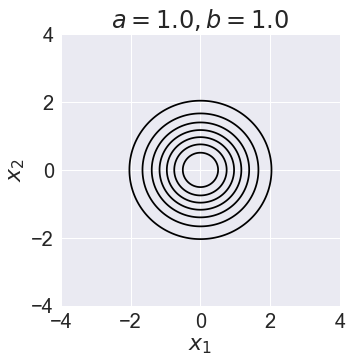
\includegraphics[width=0.24\textwidth]{gauss_scaling0.png}
	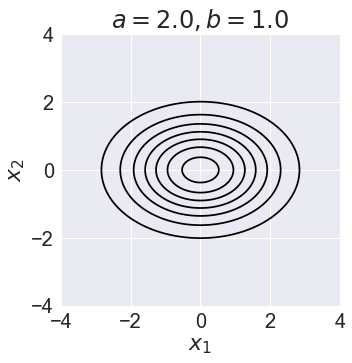
\includegraphics[width=0.24\textwidth]{gauss_scaling1.png}
	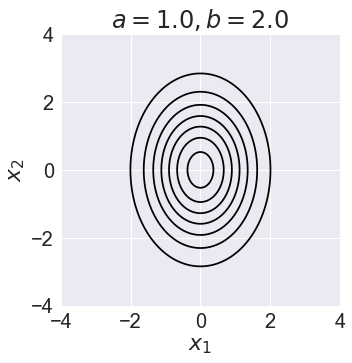
\includegraphics[width=0.24\textwidth]{gauss_scaling2.png}
	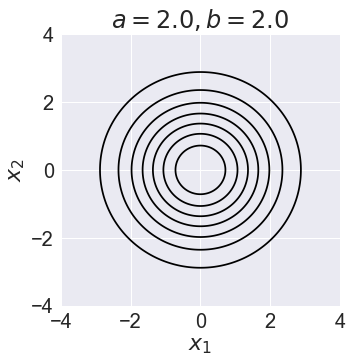
\includegraphics[width=0.24\textwidth]{gauss_scaling3.png}
	\end{center}
	\vspace*{-0.5cm}

	\pause
	
	Questions:
	\begin{enumerate}
		\item If $\bm{\Sigma}$ is diagonal, then $x_1$ and $x_2$ are uncorrelated? True or false?
		\item If $\bm{\Sigma}$ is diagonal, then $x_1$ and $x_2$ are independent? True or false?
		\item What is  the volume (integral) of density?
		\item Which of the four densities has the highest peak and why?
	\end{enumerate}
\end{frame}


\begin{frame}{More slides..}
\end{frame}


% last slide
\begin{frame}{The end of todays lecture}
\begin{itemize}
	\item Next thursday 14th, 10pm 
	\begin{itemize}
		\item We will introduce Gaussian processes more formally
		\item Read Chapter 1 \& 2 of the Gaussian process book \url{gaussianprocess.org/gpml}
	\end{itemize}

	\vspace{10mm}

	\item Time to work: first assignment
	\begin{itemize}
	    \item Released today, deadline jan 20th, 12:00 (midday)
		\item Reviews the basics of Bayesian inference and Gaussians
    	\item \textbf{Must be} handed in through MyCourses
    	\item Q\&A sessions on 20th and 22th (grants extra point for being present!)
	\end{itemize}
\end{itemize}
\end{frame}


\end{document}
